\documentclass[12pt,fullpage]{article}
\usepackage{graphicx}
\usepackage{latexsym}
\usepackage{epsfig}
\usepackage{fullpage}
\usepackage{xspace}
\usepackage{color}
\usepackage{dsfont}
\usepackage{amsmath}
\usepackage{amssymb}
\usepackage{wasysym}
\usepackage{wrapfig}
\usepackage{tikz}
\usepackage{graphicx}
\usepackage{subcaption}
\usepackage{paralist}
\usepackage{algorithm, algpseudocode}

\usepackage{enumitem}



\newcommand{\swallow}[1]{#1}

\renewcommand{\swallow}[1]{}



\usetikzlibrary{arrows}
\special{papersize=8.5in,11in}

\newcommand{\mab}[1]{{\color{red}{\bf \sf \footnotesize Michael:} \sf \scriptsize  #1}}

\newcommand{\dzejla}[1]{{\color{blue}{\bf \sf \footnotesize Dzejla:} \sf \scriptsize  #1}}

\newcommand{\twodots}{\mathinner{\ldotp\ldotp}}
\renewcommand{\epsilon}{\varepsilon}
\newcommand{\litlow}[1]{\mathord{\mathcode`\-="702D\sf #1\mathcode`\-="2200}}
\newcommand{\lit}[1]{\ensuremath{\litlow{#1}}}

\newcommand{\defn}[1] {{\textit{\textbf{\myboldmath #1\/}}}}
\newcommand{\myboldmath}{\boldmath}

\newcommand{\junk}[1]{}




\newtheorem{theorem}            {Theorem}
\newtheorem{claim}[theorem]     {Claim}
\newtheorem{xample}             {Example}
\newenvironment{example}        {\begin{xample}\rm}{\end{xample}}


\DeclareGraphicsExtensions{.pdf,.png,.jpg}




\def\compactify{\itemsep=0pt \topsep=0pt \partopsep=0pt \parsep=0pt}
\let\latexusecounter=\usecounter
\newenvironment{CompactItemize}
  {\def\usecounter{\compactify\latexusecounter}
   \begin{itemize}}
  {\end{itemize}\let\usecounter=\latexusecounter}
\newenvironment{CompactEnumerate}
  {\def\usecounter{\compactify\latexusecounter}
   \begin{enumerate}}
  {\end{enumerate}\let\usecounter=\latexusecounter}


\let\latexcite=\cite
\def\cite{\nolinebreak\latexcite}
\let\latexref=\ref
\def\ref{\nolinebreak\latexref}





\iffalse
\newcommand{\algorithm}[1]{

{\rm
\begin{center}
\begin{tabbing}
while \= while \= while \= while \= while \= while \= while \= while \= \kill
#1
\end{tabbing}
\end{center}
}

}
\fi

\newcounter{problemctr}
\addtocounter{problemctr}{0}


\newcounter{totalpoints}
\newcounter{totaltime}

\newcommand{\docounters}[3]{
    \newcounter{#1}
    \addtocounter{#1}{#2}


    \newcounter{#1time}
    \addtocounter{#1time}{#3}


    \addtocounter{totalpoints}{#2}
    \addtocounter{totaltime}{#3}
}













\newcommand{\newproblem}[5]{
    \newcommand{#1} {
        \newpage
        \addtocounter{problemctr}{1}
        \noindent
        {\bf Problem \theproblemctr.  (#3\xspace points)}
        \swallow{ (#4\xspace minutes)}

        \smallskip
        #5
    }
    \addtocounter{totalpoints}{#3}
    \addtocounter{totaltime}{#4}
    \newcommand{#2}{#3}
}















\newcounter{namesign}
\addtocounter{namesign}{2} 
\addtocounter{totalpoints}{\thenamesign}



\docounters{truefalse}{32}{26}
\docounters{alllanguagesregular}{16}{15}
\docounters{dfastates}{22}{15}
\docounters{insert}{14}{25}
\docounters{morealessb}{14}{20}



\begin{document}



{\bf
\noindent
CSE 350 --  Honors Theory of Computation\hfill             Midterm Exam\\
Michael A. Bender\hfill      April 5, 2018\\
}
\rule{\linewidth}{.01in}
\begin{center}
{\bf ~~~}
\end{center}


\medskip

Name: \rule{2.625in}{.01in} ID \#: \rule{2.5in}{.01in}\\[\bigskipamount]





\noindent {\bf INSTRUCTIONS:}
\begin{compactitem}
\item Except for your proofs, your answers should be at most $1$ or
  $2$ sentences (excluding work.)
\item This is a closed book, closed notes exam.
\item Check to see that you have 12 pages including this cover and
  scratch pages.

\item Read all the problems before starting work.
\item Think before you write.
\item If you leave a question blank or write just ``I do not know,''
  you get 25\
\item Good luck!!
\end{compactitem}

Academic integrity is expected of all students at all times, whether
in the presence or absence of members of the faculty.

Understanding this, I declare that I shall not give, use, or receive
unauthorized aid in this examination.  I have been warned that if I
am caught cheating (either receiving or giving unauthorized aid) I
will get a ``Q'' grade for this course, and a letter will be sent to
the Committee on Academic Standing and Appeals (CASA) requesting
that an academic dishonesty notation be placed on my transcript.
Further action against me may also be taken.



\noindent

Signature\footnote{No ``I dunno'' points for leaving this blank. \smiley} \rule{2.625in}{.01in}






\nopagebreak



\begin{center}

\begin{tabular}{||c|c|c||} \hline
Problem&Score&Maximum\\ \hline
{\small your signature}&              \hspace{0.5in}          &        \thenamesign \\ \hline
1&& \thetruefalse\\ \hline
2&& \thealllanguagesregular\\ \hline
3&& \thedfastates\\ \hline
4&& \themorealessb\\ \hline
5&& \theinsert\\ \hline
{\small extra credit}&& 10\\ \hline
 Total& &\thetotalpoints\\ \hline
\end{tabular}
\end{center}

\swallow{
Total minutes: \thetotaltime\xspace and Total points: \thetotalpoints.}





\sloppy




\newpage
\begin{center}
\textbf{Pumping Lemmas\footnote{Wasn't it nice of your prof and TAs to add
this page?   \smiley }}
\end{center}

\bigskip
\bigskip

\noindent
\textbf{Pumping Lemma for Regular Languages (Weak version)}:

\noindent
If $L$ is infinite and regular, then there exist strings $x$, $y$, and
$z$, where $y \neq \epsilon$, such that for each $n \geq 0$, $xy^nz \in L$.

\bigskip
\bigskip


\noindent
\textbf{Pumping Lemma for Regular Languages (Strong version)}:

\noindent If $L$ is infinite and regular, then there exists a constant $k$,
such that for any string $\omega \in L$ with $|\omega| \geq k$, $\omega = xyz$
where:

\noindent
\begin{enumerate}


\item $|xy| \leq k$,

\item $|y| > 0$, and

\item for all $n \geq 0$, $xy^nz \in L$.

\end{enumerate}



























\newpage
\addtocounter{problemctr}{1}
\noindent
{\bf
Problem \theproblemctr.  (\thetruefalse \xspace points)}
\swallow{ (\thetruefalsetime\xspace minutes)}
\smallskip

\noindent
\textbf{Please give a one-sentence justification for each question
	revealing your thinking.}
\\



\newcommand{\tfspacing}{\vspace{2cm}}

\begin{enumerate}[label=(\alph*) {\bf ~~~T~~~~F~~~~ },leftmargin=*]









\item If $\Sigma$ is a finite set, then $\Sigma^*$ is countable.

\textbf{True}. If we let each element in $\Sigma$ map to an integer, every word in $\Sigma^*$ will be a concatenation of integers, mapping to an element in $\mathbb{N}$.
\tfspacing

\item If $L$ and $L_1$ are regular, and $L = L_1 \cup L_2$, then $L_2$ is regular.

\textbf{False}. If $L_2$ is the union of the complement of $L_1$ and a nonregular language, $L_1\cup L_2=\Sigma^*$, which is regular.
\tfspacing

\item If $n$ is the length of a string and $m$ is the length of the pattern, then the KMP string matching algorithm runs in $O(n+m)$ steps.

\textbf{True}. Every iteration of KMP increments either the progress reading through the input string by 1 or the prograss reading through the pattern by 1.
\tfspacing

\item The intersection of two uncountably infinite languages could be countably infinite.

\textbf{True}. We can consider the languages representing real numbers in the ranges $\mathbb{N}\cup[0,1]$ and $\mathbb{N}\cup[1,2]$. The intersection would be the language of strings representing natural numbers, which map to their numeric forms.
\tfspacing

\item The language of strings in which the substrings ``ab'' and ``ba'' appear the same
number of times is regular.

\textbf{True}.There are a finite number of equivalence classes since the number of "ab", "ba" only differ by at most 1 assuming $\Sigma=\{a,b\}$ since any consecutive repetition of one string will generate an instance of the other.
\tfspacing

\item If there exists  $w=xyz\in L$, such that for all $n\geq0$, $xy^nz \in L$, then $L$ is regular.

\textbf{False}. Let $L=xy^*z\cup a^nb^n$ - since $a^nb^n$ is not regular, the subset of the language recognized by that pattern is not representable by a DFA, meaning L is not regular.
\tfspacing

\item There are countably many regular languages on a fixed alphabet.

\textbf{True}. A regular language can be represented by a regular expression, and since the number of characters in a regular expression is finite and the size of the expression is finite, the number of regular expressions using an alphabet and the number of regular languages on it are countably infinite.
\tfspacing

\item   In class we saw that if you take a homing sequence and tack extra characters onto the end, it stays a homing sequence.  Suppose that you tack them onto the beginning instead.  You still have a homing sequence.

\textbf{True}. Homing sequences work regardless of where one starts - it only matches a unique output to some final state and prepending characters to the beginning doesn't disrupt the mapping of unique outputs to final states.

\end{enumerate}













\newpage
\addtocounter{problemctr}{1}
\noindent
{\bf
Problem \theproblemctr.  (\thealllanguagesregular \xspace points)}
\swallow{ (\thealllanguagesregulartime\xspace minutes)}

\smallskip

\noindent
Given below is a proof to show that all languages are regular. State very
clearly and explicitly what is wrong with the following proof and why.
\bigskip\bigskip

The proof is by induction on the size of the language.

\bigskip

{\bf Base cases:} $n \in \{ 0, 1 \}$

The empty set is a regular language, and any one-element set is a regular language. Therefore every language of size $0$ or $1$ is regular.

\bigskip

{\bf Inductive step:} Assume that all languages of size $n$ are regular. Let $L$ be any language of size $n+1$, and choose some string $w \in L$. Then $|L-\{w\}| = n$, so by the inductive hypothesis, $L-\{w\}$ is regular. Since $L = \{w\} \cup (L-\{w\})$ and regular languages are closed under union, $L$ is regular. Since we assumed nothing about $L$ other than its size, any language of size $n+1$ is regular.

\bigskip

Therefore, by induction, all languages are regular.

\bigskip

The problem with this proof is that it does not take into account countably infinite languages where we can't simply assume a size $(\infty-1)$ language is regular to prove a size $\infty$ language is also regular since both are essentially equivalent.
\
\newpage
\addtocounter{problemctr}{1}
\noindent
{\bf
Problem \theproblemctr.  (\thedfastates \xspace points)}
\swallow{ (\thedfastatestime\xspace minutes)}

\smallskip

\noindent Let $L$ = $b^*a^*$. Please draw a DFA for $L$ below.

\vspace*{6em}
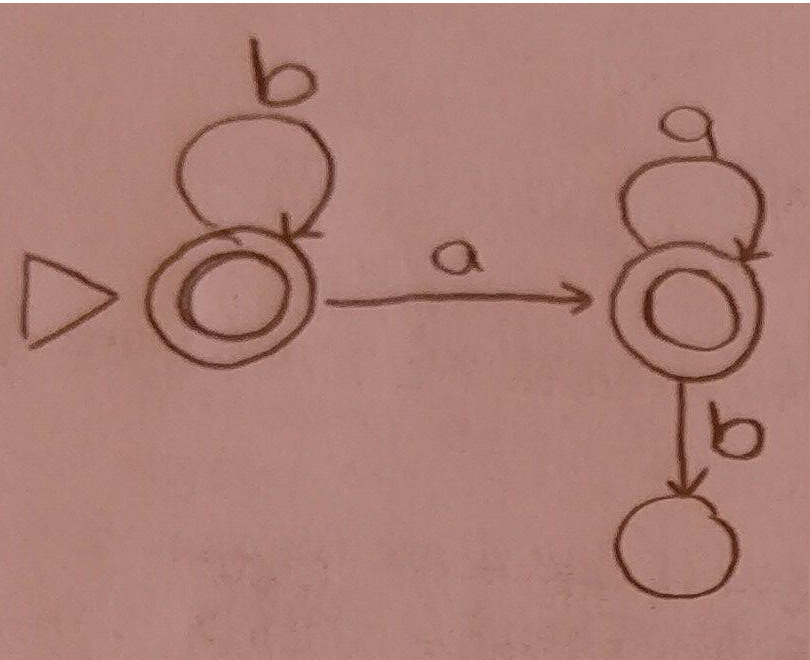
\includegraphics[scale=0.25]{dfa.jpg}
\vspace*{6em}


\noindent How many equivalence classes for $L$ are there?
\rule{1cm}{.01in}3\rule{1cm}{.01in}

\bigskip

\noindent
Please list them below.

\bigskip


\rule{2cm}{.01in}$[b^*],[bb*a],[\Sigma^*a\Sigma^*b\Sigma^*]$\rule{2cm}{.01in}

\bigskip

\noindent Use your findings above to prove that any DFA for L must have at least two
accepting states.


If we assume for sake of contradiction that L has fewer than 2 accepting states:
\begin{itemize}
    \item there can't be 0 accepting states because at least one string (ba) is in the language
    \item If there is 1 state, the for any string accepted by the DFA, the same transition will bring both to the same state. However, 'b' and 'ba' are both in the language and should be part of the same state - appending 'b' to both yields $'bb'\in L$ and $'bab'\not\in L$, a contradiction that proves the assumption false.
\end{itemize}












\newpage
\addtocounter{problemctr}{1}
\noindent
{\bf
Problem \theproblemctr.  (\theinsert \xspace points)}
\swallow{ (\theinserttime\xspace minutes)}

\smallskip

\noindent
Let $L_1$ and $L_2$ be languages.
Let
\(
\mbox{\textit{INSERT}}(L_1, L_2) =
\{w = xyz \mid xz \in L_1 \mbox{ and } y \in L_2\}
\).

\bigskip

\noindent Suppose that $L_1$ and $L_2$ are regular and have the following DFA's:

\bigskip

\begin{figure}[h]
$L_{1}$~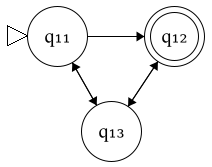
\includegraphics[scale=.5]{dfa1.png}~~~~~~~~~~~~~~~~~~~~~~$L_2$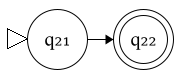
\includegraphics[scale=.5]{dfa2.png}
\centering
\end{figure}


\noindent Below is a partial construction of an NDFA that recognizes $INSERT(L_1,L_2)$. Complete the construction by marking the start state, adding the missing $\epsilon$-transitions, and circling any accept states. \footnote{It turns out you can generalize this procedure to work for any two DFAs. This means that regular languages are closed under the INSERT operation!}

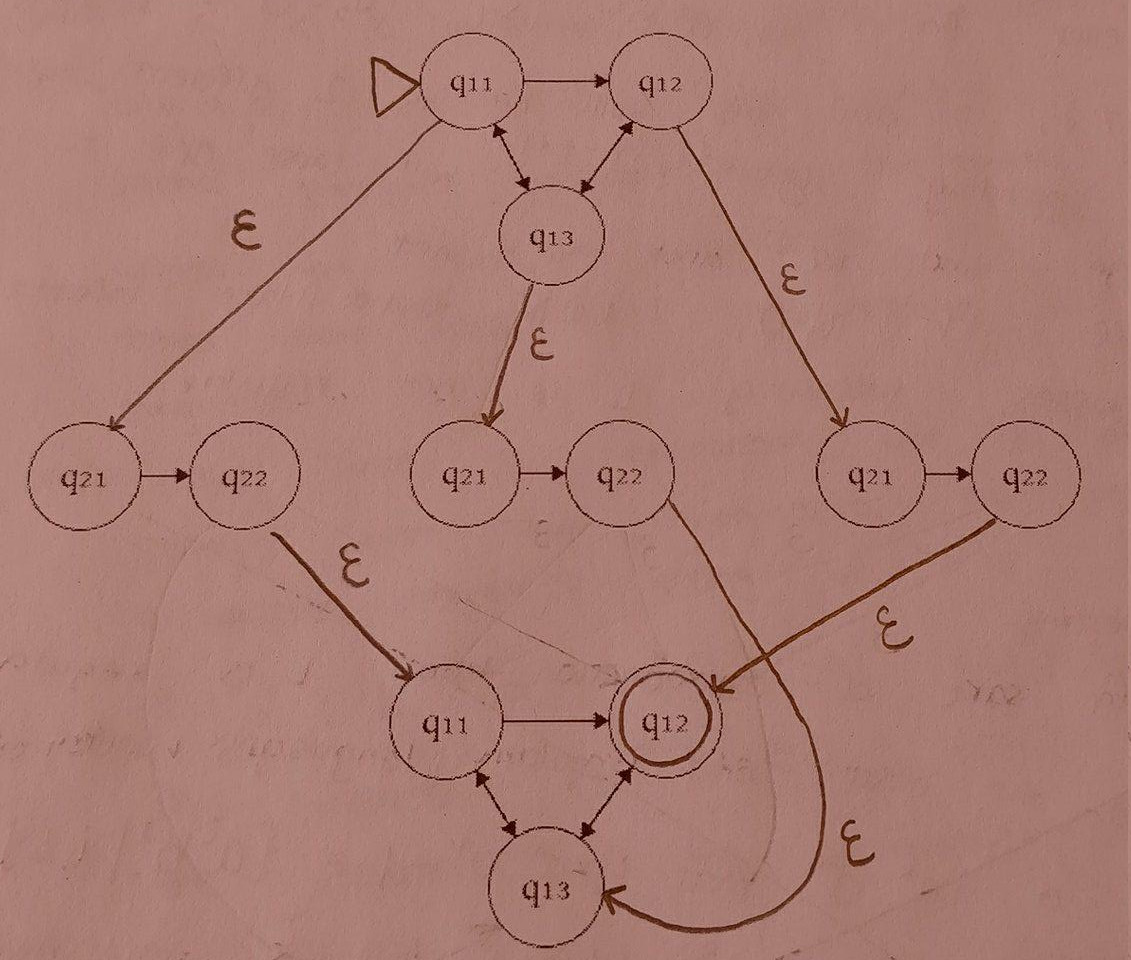
\includegraphics[scale=.4]{insert.jpg}


\iffalse
Using the DFA's for regular languages $L_1$ and $L_2$, this question explores how to construct an NDFA that recognizes $\mbox{\textit{INSERT}}(L_1, L_2)$.

\vspace*{2em}
\noindent
If the DFA for $L_1$ has $k$ states and the DFA for $L_2$ has $\ell$ states, please give your best approximation of the number of states in the NDFA you constructed.

~

\rule{5cm}{.01in}


\bigskip\bigskip\bigskip\bigskip\bigskip

Please try to explain your construction in words \emph{and} with a little sketch.
\fi







\newpage
\addtocounter{problemctr}{1}
\noindent
{\bf
Problem \theproblemctr.  (\themorealessb \xspace points)}
\swallow{ (\themorealessbtime\xspace minutes)}

\smallskip

\noindent
In class, we learned several methods to prove that a language is non-regular. Using \textbf{one of the three} methods given below, show that the language $L = \{a^nb^t | n \ge t\}$ is NOT regular. Indicate your choice by writing a checkmark on the line provided.

\bigskip

For each additional proof you provide, you will get \textbf{$5$ points of extra credit}. Clearly indicate which proof method(s) you are using for extra credit by writing ``EC'' on the line provided.

\bigskip

\begin{enumerate}
\item[\rule{1cm}{.01in}   a)] Distinguishability / Myhill-Nerode Theorem\\

By the Myhill Nerode Theorem, a language is regular if and only if there are finite equivalence classes.\\
However, for $w_1=a^ib^t, i\geq t, w_2=a^jb^t, j\geq t$, if $i\neq j$, $w_1$ and $w_2$ will be in 2 different equivalence classes since appending $b^{max\{i,j\}-t+1}$ will cause one to be in the language and the other to not be in the language.\\
Since for $t=0, i,j\in\mathbb{N}$, there are infinite equivalence classes meaning L is not regular.

\item[\rule{1cm}{.01in}   b)] Closure Properties

\vspace{0.33\textheight}

\newpage
\item[\rule{1cm}{.01in}   c)] Pumping Lemma (indicate which version you are using)

This will be a proof by contradiction.\\
We will assume for sake of contradiction that $L=\{a^nb^t|n\geq t\}$ is regular.\\
By the strong pumping lemma, there exists a value k for all strings w such that $|w|\geq k$, $w=xyz$, $|xy|\leq k$, $|y|>0$, and $\forall n\geq 0, xy^nz\in L$ where $n\geq 0$.\\
Since k is a constant, we pick a string in the language, $w=a^kb^k$ Since $|w|>k$, by the strong pumping lemma, some nonempty substring occurring within the first k characters can be repeated $n$ times where $n\geq0$ and the string will be in the language.\\
Since the first $k$ characters are 'a' and the pumping string must be nonzero, the pumping string is a nonzero, length-$p$ string of 'a's. By the lemma, $xy^nz\in L$ for $n\geq 0$. So $xy^0z\in L$. This means $a^{k-p}b^k\in L, p>0$. This contradicts the definition of the language which states $n\geq t$.\\
So we have roven though contradiction L is not regular.
\end{enumerate}








\newpage
{\bf \begin{center} Scratch Paper


\newpage
Scratch Paper


\newpage
Scratch Paper






\end{center}}

\end{document}
